%%%%%%%% ICML 2020 EXAMPLE LATEX SUBMISSION FILE %%%%%%%%%%%%%%%%%

\documentclass{article}

% Custom packages
\usepackage{amsthm}
\usepackage{amsmath}
\usepackage{amssymb}
\usepackage{blkarray}
\usepackage{todonotes}
\usepackage{mathtools}


%%%%%%%%%%%%%%%%%%%%%%%%%%%%
% Paper dependent stuff    %
%%%%%%%%%%%%%%%%%%%%%%%%%%%%

\newcommand{\Tau}{\mathcal{T}}

%%%%%%%%%%%%%%%%%%%%%%%%%%%%
% Aesthetics               %
% over-underline, hat, bold%
%%%%%%%%%%%%%%%%%%%%%%%%%%%%

\newcommand{\eps}{\varepsilon}
\newcommand{\vareps}{\varepsilon}
\renewcommand{\epsilon}{\varepsilon}
%\renewcommand{\hat}{\widehat}
\renewcommand{\tilde}{\widetilde}
\renewcommand{\bar}{\overline}

\newcommand*{\MyDef}{\mathrm{\tiny def}}
\newcommand*{\eqdefU}{\ensuremath{\mathop{\overset{\MyDef}{=}}}}% Unscaled version
% \newcommand*{\eqdef}{\mathop{\overset{\MyDef}{\resizebox{\widthof{\eqdefU}}{\heightof{=}}{=}}}}
\newcommand{\eqdef}{\stackrel{def}{=}}


\def\:#1{\protect \ifmmode {\mathbf{#1}} \else {\textbf{#1}} \fi}
\newcommand{\CommaBin}{\mathbin{\raisebox{0.5ex}{,}}}

\newcommand{\wt}[1]{\widetilde{#1}}
\newcommand{\wh}[1]{\widehat{#1}}
\newcommand{\wo}[1]{\overline{#1}}
\newcommand{\wb}[1]{\overline{#1}}

% bf and bm missing due to conflict!!
\newcommand{\bsym}[1]{\mathbf{#1}}
\newcommand{\bzero}{\mathbf{0}}
\newcommand{\ba}{\mathbf{a}}
\newcommand{\bb}{\mathbf{b}}
\newcommand{\bc}{\mathbf{c}}
\newcommand{\bd}{\mathbf{d}}
\newcommand{\be}{\mathbf{e}}
\newcommand{\bg}{\mathbf{g}}
\newcommand{\bh}{\mathbf{h}}
\newcommand{\bi}{\mathbf{i}}
\newcommand{\bj}{\mathbf{j}}
\newcommand{\bk}{\mathbf{k}}
\newcommand{\bl}{\mathbf{l}}
\newcommand{\bn}{\mathbf{n}}
\newcommand{\bo}{\mathbf{o}}
\newcommand{\bp}{\mathbf{p}}
\newcommand{\bq}{\mathbf{q}}
\newcommand{\br}{\mathbf{r}}
\newcommand{\bs}{\mathbf{s}}
\newcommand{\bt}{\mathbf{t}}
\newcommand{\bu}{\mathbf{u}}
\newcommand{\bv}{\mathbf{v}}
\newcommand{\bw}{\mathbf{w}}
\newcommand{\bx}{\mathbf{x}}
\newcommand{\by}{\mathbf{y}}
\newcommand{\bz}{\mathbf{z}}

\newcommand{\bA}{\mathbf{A}}
\newcommand{\bB}{\mathbf{B}}
\newcommand{\bC}{\mathbf{C}}
\newcommand{\bD}{\mathbf{D}}
\newcommand{\bE}{\mathbf{E}}
\newcommand{\bF}{\mathbf{F}}
\newcommand{\bG}{\mathbf{G}}
\newcommand{\bH}{\mathbf{H}}
\newcommand{\bI}{\mathbf{I}}
\newcommand{\bJ}{\mathbf{J}}
\newcommand{\bK}{\mathbf{K}}
\newcommand{\bL}{\mathbf{L}}
\newcommand{\bM}{\mathbf{M}}
\newcommand{\bN}{\mathbf{N}}
\newcommand{\bO}{\mathbf{O}}
\newcommand{\bP}{\mathbf{P}}
\newcommand{\bQ}{\mathbf{Q}}
\newcommand{\bR}{\mathbf{R}}
\newcommand{\bS}{\mathbf{S}}
\newcommand{\bT}{\mathbf{T}}
\newcommand{\bU}{\mathbf{U}}
\newcommand{\bV}{\mathbf{V}}
\newcommand{\bW}{\mathbf{W}}
\newcommand{\bX}{\mathbf{X}}
\newcommand{\bY}{\mathbf{Y}}
\newcommand{\bZ}{\mathbf{Z}}

% calligraphic
\newcommand{\cf}{\mathcal{f}}
\newcommand{\cA}{\mathcal{A}}
\newcommand{\cB}{\mathcal{B}}
\newcommand{\cC}{\mathcal{C}}
\newcommand{\cD}{\mathcal{D}}
\newcommand{\cE}{\mathcal{E}}
\newcommand{\cF}{\mathcal{F}}
\newcommand{\cG}{\mathcal{G}}
\newcommand{\cH}{\mathcal{H}}
\newcommand{\cI}{\mathcal{I}}
\newcommand{\cJ}{\mathcal{J}}
\newcommand{\cK}{\mathcal{K}}
\newcommand{\cL}{\mathcal{L}}
\newcommand{\cM}{\mathcal{M}}
\newcommand{\cN}{\mathcal{N}}
\newcommand{\cO}{\mathcal{O}}
\newcommand{\cP}{\mathcal{P}}
\newcommand{\cQ}{\mathcal{Q}}
\newcommand{\cR}{\mathcal{R}}
\newcommand{\cS}{\mathcal{S}}
\newcommand{\cT}{\mathcal{T}}
\newcommand{\cU}{\mathcal{U}}
\newcommand{\cV}{\mathcal{V}}
\newcommand{\cW}{\mathcal{W}}
\newcommand{\cX}{\mathcal{X}}
\newcommand{\cY}{\mathcal{Y}}
\newcommand{\cZ}{\mathcal{Z}}

%%%%%%%%%%%%%%%%%%%%%%%%%%%%
% Math jargon              %
%%%%%%%%%%%%%%%%%%%%%%%%%%%%
\newcommand{\wrt}{w.r.t.\xspace}
\newcommand{\defeq}{\stackrel{\mathclap{\normalfont\mbox{\tiny def}}}{=}}
\newcommand{\maxund}[1]{\max\limits_{#1}}
\newcommand{\supund}[1]{\text{sup}\limits_{#1}}
\newcommand{\minund}[1]{\min\limits_{#1}}
\renewcommand{\epsilon}{\varepsilon}
\newcommand{\bigotime}{\mathcal{O}}


\DeclareMathOperator*{\argmin}{arg\,min} 
\DeclareMathOperator*{\argmax}{arg\,max} 
\DeclareMathOperator*{\cupdot}{\mathbin{\mathaccent\cdot\cup}}

%%%%%%%%%%%%%%%%%%%%%%%%%%%%
% Matrix operators         %
%%%%%%%%%%%%%%%%%%%%%%%%%%%%
\newcommand{\transpose}{^\mathsf{\scriptscriptstyle T}}
\newcommand{\transp}{\mathsf{\scriptscriptstyle T}}
\DeclareMathOperator{\Tr}{Tr}
\DeclarePairedDelimiterX{\inp}[2]{\langle}{\rangle}{#1, #2}

%%%%%%%%%%%%%%%%%%%%%%%%%%%%
% Statistic operators      %
%%%%%%%%%%%%%%%%%%%%%%%%%%%%
\newcommand{\probability}[1]{\mathbb{P}\left(#1\right)}
\newcommand{\probdist}{Pr}
\DeclareMathOperator*{\expectedvalue}{\mathbb{E}}
\DeclareMathOperator*{\variance}{\text{Var}}
\newcommand{\expectedvalueover}[1]{\expectedvalue\limits_{#1}}
\newcommand{\condbar}{\;\middle|\;}
\newcommand{\gaussdistr}{\mathcal{N}}
\newcommand{\uniformdistr}{\mathcal{U}}
\newcommand{\bernoullidist}{\mathcal{B}}

%%%%%%%%%%%%%%%%%%%%%%%%%%%%
% Algebraic Sets           %
%%%%%%%%%%%%%%%%%%%%%%%%%%%%
\newcommand{\Real}{\mathbb{R}}
\newcommand{\Natural}{\mathbb{N}}
\newcommand{\statespace}{\mathcal{X}}
\newcommand{\funcspace}{\mathcal{F}}
\newcommand{\dynaspace}{\mathcal{T}}


\newtheorem{theorem}{Theorem}
\newtheorem{definition}{Definition}
\newtheorem{lemma}{Lemma}
\newtheorem{proposition}{Proposition}
\providecommand*\propositionautorefname{Proposition}
\newtheorem{remark}{Remark}
\newtheorem{property}{Property}
\newtheorem{assumption}{Assumption}
\providecommand*\assumptionautorefname{Assumption}
\newtheorem{conjecture}{Conjecture}

\newtheorem*{definition*}{Definition}
\newtheorem*{theorem*}{Theorem}
\newtheorem*{proposition*}{Proposition}
\newtheorem*{remark*}{Remark}
\newtheorem*{example*}{Example}

% Recommended, but optional, packages for figures and better typesetting:
\usepackage{microtype}
\usepackage{graphicx}
\usepackage{subfigure}
\usepackage{booktabs} % for professional tables

% hyperref makes hyperlinks in the resulting PDF.
% If your build breaks (sometimes temporarily if a hyperlink spans a page)
% please comment out the following usepackage line and replace
% \usepackage{icml2020} with \usepackage[nohyperref]{icml2020} above.
\usepackage{hyperref}

% Attempt to make hyperref and algorithmic work together better:
\newcommand{\theHalgorithm}{\arabic{algorithm}}

% Use the following line for the initial blind version submitted for review:
\usepackage{icml2020}

% If accepted, instead use the following line for the camera-ready submission:
%\usepackage[accepted]{icml2020}

% The \icmltitle you define below is probably too long as a header.
% Therefore, a short form for the running title is supplied here:
\icmltitlerunning{Robust Estimation, Prediction and Control}

\begin{document}
	
	\twocolumn[
	\icmltitle{Robust Estimation, Prediction and Control with \\ Linear Dynamics and Arbitrary Costs}
	
	% It is OKAY to include author information, even for blind
	% submissions: the style file will automatically remove it for you
	% unless you've provided the [accepted] option to the icml2020
	% package.
	
	% List of affiliations: The first argument should be a (short)
	% identifier you will use later to specify author affiliations
	% Academic affiliations should list Department, University, City, Region, Country
	% Industry affiliations should list Company, City, Region, Country
	
	% You can specify symbols, otherwise they are numbered in order.
	% Ideally, you should not use this facility. Affiliations will be numbered
	% in order of appearance and this is the preferred way.
	\icmlsetsymbol{equal}{*}
	
	\begin{icmlauthorlist}
		\icmlauthor{Edouard Leurent}{seq,val,ren}
		\icmlauthor{Denis Efimov}{val}
		\icmlauthor{Odalric Ambrym-Maillard}{seq}
	\end{icmlauthorlist}
	
	\icmlaffiliation{seq}{Inria Lille Nord-Europe, Sequel Project, Lille, France}
	\icmlaffiliation{val}{Inria Lille Nord-Europe, Valse Project, Lille, France}
	\icmlaffiliation{ren}{Renault Group, Guyancourt, France}
	
	\icmlcorrespondingauthor{Edouard Leurent}{edouard.leurent@inria.fr}
	
	% You may provide any keywords that you
	% find helpful for describing your paper; these are used to populate
	% the "keywords" metadata in the PDF but will not be shown in the document
	\icmlkeywords{Machine Learning, ICML}
	
	\vskip 0.3in
	]
	
	% this must go after the closing bracket ] following \twocolumn[ ...
	
	% This command actually creates the footnote in the first column
	% listing the affiliations and the copyright notice.
	% The command takes one argument, which is text to display at the start of the footnote.
	% The \icmlEqualContribution command is standard text for equal contribution.
	% Remove it (just {}) if you do not need this facility.
	
	\printAffiliationsAndNotice{}  % leave blank if no need to mention equal contribution
%	\printAffiliationsAndNotice{\icmlEqualContribution} % otherwise use the standard text.
	
\begin{abstract}
	We develop a framework for the adaptive control of a linear system with unknown parameters and arbitrary costs in a critical setting where failures are costly and should be prevented at all time. We build on two ideas: first, we incorporate prior knowledge of the dynamics in the form of a known structure of the uncertainty, which can be tightened as we collect interaction data by building high-confidence regions through least-square regression. Second, we act in a cautious way with respect to this uncertainty by formulating a robust objective, that we solve approximately in a prediction-optimisation manner, leveraging tools from interval prediction and sequential planning literatures. Additionally, we relax our modelling assumptions by proposing an extension based on multi-model selection and aggregation. The full procedure is designed to produce reasonable and safe behaviour at deployment, get more aggressive with time, and be asymptotically optimal. We illustrate it on a practical case of autonomous driving at an intersection.
\end{abstract}	

\section{Introduction}

Despite the dazzling successes of Reinforcement learning in cracking many problems considered unsolvable in the past decade [ref needed], this tool has hardly been applied in real industrial issues. This could be attributed to two undesirable properties which limit its practical applications: the dependence on a tremendous amount of interaction data that cannot always be simulated, and the reliance on trial-and-error and random exploration. In this paper, we consider the problem of controlling an unknown linear system $x(t)$ so as to maximise an \emph{arbitrary} bounded reward function $R$, in a critical setting where mistakes are costly and must be avoided at all time. 
This choice of the rich reward space is crucial to have sufficient flexibility to model non-convex and non-smooth functions that naturally arise in many practical problems such as combinatorial optimisation, obstacle avoidance, etc. 

Since experiencing failures is out of question, the only way to prevent them from the outset, when the system is first deployed, is to rely on some sort of prior knowledge. In this work, we assume that the system dynamics are partially known, in the form of a parametrized dynamical system with unknown parameters. We argue that this assumption is realistic given that most industrial applications to date have been relying on physical models to describe their processes and engineered controllers to operate them, rather than machine learning. Our framework relaxes this modelling effort by allowing some structured uncertainty around the nominal model. We adopt a data-driven scheme where we wish to estimate the parameters more accurately as we interact with our true system. Most model-based reinforcement learning algorithms only rely on the estimated dynamics to derive the corresponding optimal controller, but these methods often suffer from \emph{model bias}: they ignore the error that exists between the learned and true dynamics, which can dramatically degrade the control performances \citep{Schneider1997}.

To address this issue, we turn to the framework of \emph{robust} decision-making: instead of merely considering a point estimate of the dynamics, we build an entire \emph{confidence region} that contains the true dynamics with high probability, and optimise the decisions so as to maximise the worst-case outcome with respect to this uncertainty. Minimax problem are hard to solve, especially since $R$ can be arbitrary. We cannot use traditional tools from the robust LQ control community (coarse-id control, system-level synthesis). Instead, we adopt a hierachical control architecture, controller selection: discrete choice of a driving maneuver, a short-term goal, whose execution is performed by a fixed low-level controller. It is true that the passage from continuous optimization to discrete optimization induces a suboptimality. However, it can be mitigated by using a more diverse controller basis. We are left with a sequential optimization problem with continuous states and discrete actions: tree-based planning algorithms. But not a point estimate, a whole confidence region. Hence, a two step procedure: robust prediction of the reachability set, which provides a conservative pessimistic reward to the planning algorithm.


\subsection{Problem Statement and Our Contributions}

\paragraph{Notations}

The dynamics of the real system are described in continuous time. However, all the sensing and control performed on-board happen in discrete time, with time-step $\dd t$. For any variable $z$, we use the subscript notation to refer to these discrete times: $z_n = z(t_n)$ with $t_n = n\dd t$.

\paragraph{Structured dynamics}
We consider a linear system with state $x\in\Real^p$, acted on by controls $u\in\Real^q$ and perturbations $\omega\in\Real^r$, and following a dynamics in the form:

\begin{equation}
\label{eq:dynamics}
\dot{x}(t)=A(\theta)x(t) + B u(t) + D \omega(t),\;t\geq0.
\end{equation}
The dynamics $A(\theta)\in\Real^{p\times p}$  depends on some parameter $\theta$ that belongs to a compact set $\Theta \subset \Real^d$. The control matrix $B\in\Real^{p\times q}$ and disturbance matrix $D\in\Real^{p\times r}$ are known.

We also have access to the observation of $x(t)$ and to a noisy measurement of $\dot{x}(t)$ in the form $\dot{x}(t) + C\nu(t)$, where $\nu(t)\in\Real^s$ is a measurement noise and $C\in\Real^{p\times s}$ is known. Assumptions over the disturbance $\omega$ and noise $\nu$ will be detailed further, and we denote $\eta(t) = C\nu(t) + D\omega(t)$.

\paragraph{Model estimation}

In \autoref{sec:estimation}, having observed history of transitions $\cD_{[N]} = \{(x_n, u_n, y_n)\}_{n\in[N]}$, and given a confidence level $\delta\in(0, 1)$, our goal is to find a confidence region $\cC_{[N],\delta}$ as tight as possible and such that it holds that:
\begin{align}
\probability{A(\theta)\in \cC_{[N],\delta}} \geq 1-\delta
\label{eq:polytope}
\end{align}
Our first contribution is to extend the work of \citet{Abbasi2011} that provide a confidence ellipsoid for the regularised least-square estimator in the case of scalar noise and vector features to our setting of vector noise and matrix features.

\paragraph{Robust objective}

At the time step $n=N$, considering the model uncertainty $\cC_{[N],\delta}$ obtained in the model estimation phase, we formulate our robust control objective:
\begin{equation}
\label{eq:robust-control}
\sup_{\bu\in{(\Real^q)}^\Natural} \underbrace{\inf_{\substack{A(\theta) \in \cC_{[N],\delta} \\ \bw\in[\underline{\bw},\overline{\bw}]^\Natural}} \left[\sum_{n=N+1}^\infty \gamma^n R(x_n(\bu,\bw))\right]}_{V^r(\bu)}
\end{equation}
where $\bu = (u_{N+1},u_{N+2},\cdots)$ and $\bw = (\omega_N, \omega_{N+1},\cdots)$ are the sequences of future controls and perturbations, respectively.

The rest of the paper will tackle the optimisation of this objective.

\paragraph{State prediction}

Minimax problems such as \eqref{eq:robust-control} are notoriously difficult to solve even in cases such as Linear-Quadratic systems (LQ) where the reward $R$ has a simple form. Here with an arbitrary function $R$, we cannot hope to derive a solution in explicit form. Our second contribution is to propose to solve \eqref{eq:robust-control} numerically by adopting a \emph{predict-then-optimise} scheme. Thus, in \autoref{sec:prediction}, as illustrated in \autoref{fig:interval-hull}, we aim to derive a \emph{set predictor} $X(t)$ for the system \eqref{eq:dynamics}, which takes the information on the observed current state ${x}_N$, a confidence region $\cC_\delta$ containing $A(\theta)$, a planned control sequence $\bu$ and some admissible bounds on the perturbation $[\underline{\omega}(t),\overline{\omega}(t)]$; and verifies the inclusion property:
\begin{equation}
 x(t)\in X(t),\quad\forall t\geq t_N.
\end{equation}

\begin{figure}
    \centering
    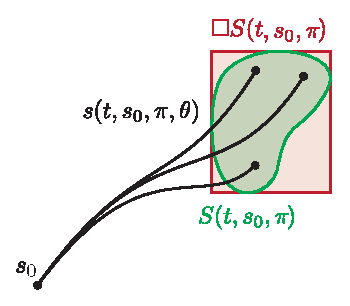
\includegraphics[width=0.3\textwidth]{img/interval-hull}
    \caption{A few trajectories are sampled from an initial state $x_N$ following controls $\bu=(u_0,\cdots)$ with various parameters $A(\theta)\in\cC_{[N],\delta}$ (in black). At time $t\geq t_N$, any reachable state $x(t)$ (in green) must belong to the candidate set predictor $X(t)$ (in red).}
    \label{fig:interval-hull}
\end{figure}

We leverage recent results from the uncertain system simulation literature to efficiently compute such a predictor.

\paragraph{Robust planning}

Since $R$ is arbitrary, solving the optimal -- not to mention the robust -- control objective in the original continuous control space $(\Real q)^\Natural$ is intractable.
In this work, we choose to approximate the solution by turning the continuous optimisation problem \eqref{eq:robust-control} into a discrete one, by optimising over a finite set of \emph{actions} $\cA$. Each action $a\in\cA$ corresponds to the selection of a low-level controller $\pi_a$, that we take affine:
\[u(t) = \pi_a(x(t)) \eqdef -K_a x(t) + u_a\]

The robust objective we consider becomes 
\begin{equation}
\label{eq:robust-control-disc}
\sup_{\ba\in{\cA}^\Natural} \underbrace{\inf_{\substack{A(\theta) \in \cC_{[N],\delta} \\ \bw\in[\underline{\bw},\overline{\bw}]^\Natural}} \left[\sum_{n=N+1}^\infty \gamma^n R(x_n(\ba,\bw))\right]}_{V^r(\ba)}
\end{equation}
where $x_n(\ba, \bw)$ is obtained by integrating \eqref{eq:dynamics} with $u_n = \pi_{a_n}(x_n)$.

In \autoref{sec:control}, facing an optimisation problem with continuous states and discrete actions, we turn to the literature of tree-based planning. Our third contribution proposes to approximate the true robust objective ${V}^r$ by an easily-evaluable surrogate $\hat{V}^r$ that exploits the set predictor to define a pessimistic reward, used to evaluate sequences of actions in a tree-based planning algorithm. We show that 


% \paragraph{Objective}

% We wish to find a sequence of commands $\bu=(u_t)_{t\geq 0}$ that maximises a cumulative objective $V^\bu$:

% \todo[inline]{EL: the prediction is done in continuous time and the control in discrete time. How to handle the change in notations?}

% \begin{equation}
% \max_\bu V^\bu
% \end{equation}
% where
% \begin{equation}
% \label{eq:optimal-control}
% V^\bu = \expectedvalueover{\omega(t)}\left[\sum_{t=0}^\infty \gamma^t r(x(t))\condbar u_t,\,\eqref{eq:dynamics}\right]
% \end{equation}
% and $r:\Real^p\rightarrow[0,1]$ is a bounded reward function.



\section{Related Work}

\paragraph{LQ systems} There is a rich body of literature dedicated to the study of LQ systems, and we focus on those providing non-asymptotic results when the system parameters $A, B$ are unknown. In their seminal work \citet{abbasi-yadkori11a}, consider the problem of cumulative regret minimisation. They follow the \emph{Optimism in the Face of Uncertainty} paradigm from the multi-armed bandit literature, that consists in selecting an optimistic system within a high-confidence region while enforcing a controllability constraint, and computing the corresponding optimal control in closed-form by solving a Riccati equation. They show that this procedures achieves a $\tilde{\cO}\left(T^{1/2}\right)$ cumulative regret. \citet{abeille18a} provide the same result by applying Thomson Sampling rather of optimism to select a dynamical model, and rejection sampling to enforce the controllability constraint.
While previous methods suffered from limited applicability and computationally intractable subroutines, \citep{Dean2018} provide a polynomial-time algorithm which achieves a suboptimal cumulative regret of $\tilde{\cO}\left(T^{2/3}\right)$.


Offline estimation and control synthesis: \citep{Dean2017}. Summary: Estimation procedure of $N$ episodes of duration $T$ with gaussian excitation, ellipsoid in L2 norm, robust controller with System Level Synthesis, simple regret in $O(\sqrt{\frac{\log(1/\delta)}{N}})$



We wish to act straight away in a reasonable (structure) but cautious (robust) way, and progressively get more and more aggressive as we obtain more data and reduce uncertainty.
    
Thus, we do not wish to explore actively the more promising regions as in OFU, nor the more likely region as in TS, nor act randomly as in Coarse-ID They inject exploration noise.
    
We have linear dynamics but our cost is not quadratic. Quadratic cost: stabilize a system around a reference trajectory known a priori. Thus, we can accurately represent planning tasks with discrete/branching decisions involving discontinuities (e.g. collision vs non-collision states).
    
Our optimisation problem amounts to a sequence of controllers selection, instead of continuous controller synthesis
    
Optimistic exploration = information seeking and uncertainty reduction. Our objective: do not commit mistakes (do not explore uncertain regions). If some information is collected allowing to reduce uncertainty, use it to be more optimal, but do not actively seek it.

Given the critical setting, we do not want to be optimistic, and try to minimise some cumulative regret. Quite the contrary, we want to be cautious, safe, prepare for the worst and plan for the best. 

\paragraph{Robust planning}
Robust optimization has been studied in the context of finite Markov Decision Processes with uncertain parameters by Iyengar (2005), Nilim and El Ghaoui (2005) and Wiesemann et al. (2013). They show that the main results of Dynamic Programming can be extended to their robust counterparts only when the dynamics ambiguity set verifies a certain rectangularity property, that amounts to an independence assumption between the uncertainty sets of each transition and is related to time-varying uncertainty.
They do not consider continuous states, nor handle time-invariant uncertainty. We do so by not relying on a dynamic programming evaluation of the robust cost-to-go, but on monte-carlo estimates along a full trajectory.

\section{Model Estimation}

\label{sec:estimation}

In the general case, 
 assume that the dynamics $A(\theta)$ enjoy the following additional structure:
\begin{assumption}[Structure]
\label{assumpt:structure}
There exists a known feature tensor $\phi\in \Real^{d \times p \times p}$ such that for all $\theta\in\Theta$:
\begin{equation}
    A(\theta) = A + %\theta^\transp \phi \eqdef A + 
    \sum_{i=1}^d \theta_i\phi_i
\end{equation}
where $\phi_i\in\Real^{p\times p}$ for all $i\in[d]$. For all $n$, we also denote $\Phi_n = [\phi_1 x_n \cdots \phi_d x_n]\in\Real^{p\times d}$.

We also assume to know an upper-bound $S$ over $\|\theta\|_\infty$.
\end{assumption}

For readability, we denote the noisy measurement of $\dot{x}$ as:
\begin{equation}
\label{eq:measurement}
    y(t) = \dot{x}(t) + C\nu(t) - A x(t) - Bu(t)
\end{equation}
which is possible since the nominal dynamics $A$, the state $x(t)$ and the control $u(t)$ are known.
Thus, we obtain the system
\[
y_n = \Phi_n\theta + \eta_n
\]

\paragraph{Regularised least square} We consider the weighted $L_2$-regularised regression problem with weights  $\Sigma_p\in\Real^{p\times p}$ and parameter $\lambda\in\Real^+_*$:


\begin{equation}
    \label{eq:regression_min}
    \min_{\theta\in\Real^d} \sum_{n=1}^N \|y_n -\Phi_n\theta\|_{\Sigma_p^{-1}}^2 + \lambda\|\theta\|_{}^2
\end{equation}


The solution can be obtained as:

\begin{proposition}[Regularised solution]
\label{prop:regularized_solution}
The solution to \eqref{eq:regression_min} is:
\begin{equation}
    \label{eq:vector_rls}
    \theta_{N,\lambda} = G_{N, \lambda}^{-1} \sum_{n=1}^N \Phi_n^\transp \Sigma_p^{-1} y_n
\end{equation}
where 
\begin{equation*}
    G_{N, \lambda} = \sum_{n=1}^N \Phi_{n}^\transp\Sigma_p^{-1}\Phi_{n}  + \lambda I_d \in \Real^{d\times d}.
\end{equation*}
\end{proposition}

By simply substituting the expression of $y_n$ into \eqref{eq:vector_rls}, we obtain the regression error:
\begin{align}
    \theta_{N,\lambda} - \theta = G_{N, \lambda}^{-1}\sum_{n=1}^N \Phi_n^\transp \Sigma_p^{-1}\eta_n - \lambda G_{N, \lambda}^{-1}\theta 
\end{align}


Depending on the assumption we have over the noise $\eta_n$, we can bound this error in different ways.


\subsection{Bounded noise}

\begin{assumption}[Bounded noise]
\label{assumpt:bounded-noise}
The noise $\eta(t)$ is bounded
\[
\|\eta\|_\infty < \infty.
\]
In particular, we denote the coefficient-wise bounds over perturbations as $\underline{\omega}(t) \leq \omega(t) \leq \overline{\omega}(t)$.
\end{assumption}

By Hölder inequality, we obtain a confidence region $\cC_\delta$ defined by a $L_1$-ball, i.e. a polytope with $2d$ vertices:
\begin{equation}
\begin{split}
\label{eq:bounded-noise-polytope}
\|\theta_{N,\lambda} - \theta\|_1 \leq {} &\|G_{N, \lambda}^{-1}\sum_{n=1}^N \Phi_n^\transp \Sigma_p^{-1}\|_1\|\eta\|_\infty \\
&+ \lambda\|G_{N, \lambda}^{-1}\|_1 S
\end{split}
\end{equation}

There may be cases where \autoref{assumpt:bounded-noise} does not hold, for instance if the noise $\eta$ is Gaussian, which implies $\|\eta\|_\infty=+\infty$ and makes \eqref{eq:bounded-noise-polytope} uninformative. Then, another weaker assumption can be made.

\subsection{Sub-Gaussian noise}

We say that a random vector $x\in\Real^k$ is sub-Gaussian with covariance proxy $\Sigma$, and denote $x\sim Sub_G(\Sigma)$, if $\expectedvalue[x] = 0_k$ and:
\[
\forall u\in\Real^k, \expectedvalue \left[ \exp{\left( u^\transp x\right)}\right] \leq \exp{\left( \frac{1}{2} u^\transp \Sigma u\right)}
\]

\begin{assumption}[Sub-Gaussian Noise]
\label{assumpt:gaussian-noise}
At each time $t\geq0$ the noise $\eta(t)$ is an independent sub-Gaussian noise with covariance proxy $\Sigma_p \in \Real^{p\times p}$:
\begin{equation*}
    \eta(t) \sim Sub_G(\Sigma_p).
\end{equation*}
For instance, this is the case when $\nu$ and $\omega$ are Gaussian noises with respective covariance matrices $\Sigma_r$ and $\Sigma_s$, with $\Sigma_p \eqdef C\Sigma_r C^\transp + D\Sigma_s D^\transp$. Also note that \autoref{assumpt:bounded-noise} implies that $\eta$ is $\|\eta\|_\infty I_p$-sub-Gaussian, and is therefore a stronger assumption.
\end{assumption}

\begin{theorem}[Confidence ellipsoid of \citep{Abbasi2011}, Matrix version]
\label{thm:confidence_ellipsoid}
Under \autoref{assumpt:gaussian-noise}, it holds with probability at least $1-\delta$ that
\begin{align}
    \label{eq:confidence-ellipsoid}
    \| \theta_{N,\lambda}  - \theta\|_{G_{N,\lambda}} \leq \beta_N(\delta),
\end{align}
with
\begin{equation}
    \beta_N(\delta)\eqdef \sqrt{2\ln \left(\frac{\det(G_{N,\lambda})^{1/2}}{\delta\det(\lambda I_d)^{1/2}}\right)}
     + (\lambda d)^{1/2}S.
\end{equation}
\end{theorem}

We can enclose this confidence ellipsoid $\eqref{eq:confidence-ellipsoid}$ into a polytope $C_\delta$. For simplicity, we present here a very simple but coarse strategy: bound the ellipsoid by its enclosing sphere, and the sphere by its enclosing hypercube:
\begin{align}
    \label{eq:generic-polytope}
     &\cC_\delta = \left\{ A_{0}+\sum_{i=1}^{2^d}\lambda_{i}\Delta A_{i}: \lambda\in[0, 1]^{2^d},  \sum_{i=1}^{2^d}\lambda_{i}=1\right\},\\
     &A_0 = A + \theta_{N,\lambda}^\transp\phi, \quad\Delta A_{i} = h_i \sqrt{\frac{\beta_N(\delta)}{\lambda_{\max}(G_{N,\lambda})}}
\end{align}

Another strategy presented in \autoref{sec:tight-polytope} produces a much tighter polytope, at the price of an increased computational cost required by the diagonalisation of $G_{N,\lambda}$.

\paragraph{Remark} The robust objective framing involves on some bounds $\underline{\omega}(t)\leq \omega(t) \leq \overline{\omega}(t)$ over the possible perturbations we want to protect against. In the unbounded sub-Gaussian noise setting of \autoref{assumpt:gaussian-noise}, we can use the same formulation by deriving high-confidence bounds that each holds with probability $\delta_t$. By choosing $\delta_t = \frac{\delta}{t(t+1)}$, we have that the event $\{\forall t, \underline{\omega}(t) \leq \omega(t) \leq \overline{\omega}(t)\}$ holds with probability $1-\delta$.

\section{State Prediction}

\label{sec:prediction}

Set representation: interval prediction

\begin{equation}
\label{eq:inclusion-property}
\underline{x}(t)\leq x(t)\leq\overline{x}(t),\quad\forall t\geq t_N.
\end{equation}

We consider interval prediction rather than zonotope prediction for instance, for the sake of simplicity of implementation and computational efficiency. 

A simple solution is proposed in \citep{efimov:hal-00701643}, where they use matrix interval arithmetics to derive the predictor:
\begin{proposition}
Assuming that \eqref{eq:polytope} is satisfied for the system \eqref{eq:dynamics}, then the interval predictor:
\begin{eqnarray}
\dot{\underline{x}}(t) & = & \underline{A}^{+}\underline{x}^{+}(t)-\overline{A}^{+}\underline{x}^{-}(t)-\underline{A}^{-}\overline{x}^{+}(t)\nonumber \\
 &  & +\overline{A}^{-}\overline{x}^{-}(t)+B^{+}\underline{d}(t)-B^{-}\overline{d}(t),\label{eq:IP_direct}\\
\dot{\overline{x}}(t) & = & \overline{A}^{+}\overline{x}^{+}(t)-\underline{A}^{+}\overline{x}^{-}(t)-\overline{A}^{-}\underline{x}^{+}(t)\nonumber \\
 &  & +\underline{A}^{-}\underline{x}^{-}(t)+B^{+}\overline{d}(t)-B^{-}\underline{d}(t),\nonumber \\
 &  & \underline{x}(0)=\underline{x}_{0},\;\overline{x}(0)=\overline{x}_{0},\nonumber 
\end{eqnarray}
ensures the inclusion property \eqref{eq:inclusion-property}.
\end{proposition}

However, \citet{leurent2019interval} showed that this predictor can have unstable dynamics, even for stable systems, which can cause a rapid build-up of uncertainty and produce over-conservative behaviours. They propose an enhanced predictor which produces tighter and more stable predictions, and whose stability can be assessed by solving a linear matrix inequality, at the price of an additional requirement:

\begin{assumption}
\label{assumpt:metzler}
There exists an orthogonal matrix $P\in\Real^{d\times d}$ such that $P^\transp A_0 P$ is Metzler, that is, all non-diagonal coefficients are non-negative.
\end{assumption}
In practice, this assumption is often verified. It is for instance the case whenever $A_0$ is diagonalisable, and a fortiori when it is stabilisable. The similarity transformation of \citep{Efimov_a2013} provides a method to compute such $P$ whenever there exist $C_1,C_2$ which make $A(\theta, C_1)$ and $(A_0, C_2)$ observable.
Under this assumption, without loss of generality up to a change of basis $x\rightarrow P^{-1}x$ that we do not write for the sake of readability, this assumption is equivalent to considering that $A_0$ itself is Metzler.

\begin{theorem}[Interval Predictor \citep{leurent2019interval}]
\label{thm:predictor}
Assuming that \eqref{eq:polytope} and \autoref{assumpt:metzler} are satisfied for the system \eqref{eq:dynamics}, then the interval predictor:
\begin{eqnarray}
\dot{\underline{x}}(t) & = & A_{0}\underline{x}(t)-\Delta A_{+}\underline{x}^{-}(t)-\Delta A_{-}\overline{x}^{+}(t)\nonumber \\
 &  & +Bu(t)+D^{+}\underline{\omega}(t)-D^{-}\overline{\omega}(t),\nonumber\\
\dot{\overline{x}}(t) & = & A_{0}\overline{x}(t)+\Delta A_{+}\overline{x}^{+}(t)+\Delta A_{-}\underline{x}^{-}(t) \label{eq:interval-predictor} \\
 &  & +Bu(t)+D^{+}\overline{\omega}(t)-D^{-}\underline{\omega}(t),\nonumber \\
 &  & \underline{x}(t_N)=\overline{x}(t_N)={x}(t_N)\nonumber 
\end{eqnarray}
ensures the inclusion property \eqref{eq:inclusion-property}.

% Moreover, the stability of the predictor can be assessed with a sufficient condition in form of an LMI.
% if there exist diagonal matrices $P$, $Q$, $Q_{+}$, $Q_{-}$, $Z_{+}$, $Z_{-}$, $\Psi_{+}$, $\Psi_{-}$, $\Psi$, $\Gamma\in\Real^{2n\times 2n}$ such that the following LMIs are satisfied:
% \begin{gather*}
% P+\min\{Z_{+},Z_{-}\}>0,\;\Upsilon\preceq0,\;\Gamma>0,\\
% Q+\min\{Q_{+},Q_{-}\}+2\min\{\Psi_{+},\Psi_{-}\}>0,
% \end{gather*}
% where{\footnotesize{}
% \begin{gather*}
% \Upsilon=\left[\begin{array}{cccc}
% \Upsilon_{11} & \Upsilon_{12} & \Upsilon_{13} & P\\
% \Upsilon_{12}^{\top} & \Upsilon_{22} & \Upsilon_{23} & Z_{+}\\
% \Upsilon_{13}^{\top} & \Upsilon_{23}^{\top} & \Upsilon_{33} & Z_{-}\\
% P & Z_{+} & Z_{-} & -\Gamma
% \end{array}\right],\\
% \Upsilon_{11}=\mathcal{A}^{\top}P+P\mathcal{A}+Q,\;\Upsilon_{12}=\mathcal{A}^{\top}Z_{+}+PR_{+}+\Psi_{+},\\
% \Upsilon_{13}=\mathcal{A}^{\top}Z_{-}+PR_{-}+\Psi_{-},\;\Upsilon_{22}=Z_{+}R_{+}+R_{+}^{\top}Z_{+}+Q_{+},\\
% \Upsilon_{23}=Z_{+}R_{-}+R_{+}^{\top}Z_{-}+\Psi,\;\Upsilon_{33}=Z_{-}R_{-}+R_{-}^{\top}Z_{-}+Q_{-},\\
% \mathcal{A}=\left[\begin{array}{cc}
% A_{0} & 0\\
% 0 & A_{0}
% \end{array}\right],\;R_{+}=\left[\begin{array}{cc}
% 0 & -\Delta A_{-}\\
% 0 & \Delta A_{+}
% \end{array}\right],\;R_{-}=\left[\begin{array}{cc}
% \Delta A_{+} & 0\\
% -\Delta A_{-} & 0
% \end{array}\right],
% \end{gather*}
% }then the predictor \eqref{eq:interval-predictor} is input-to-state stable with respect to the inputs $\underline{\omega}$, $\overline{\omega}$.
\end{theorem}

% \begin{example*}
% Consider a scalar system:
% \[
% \dot{x}(t)=-\theta(t)x(t)+d(t),\;t\geq0,
% \]
% where $x(t)\in\Real$ with $x(0)\in[\underline{x}_{0},\overline{x}_{0}]=[1.0, 1.1]$, $\theta(t)\in\Pi=[\underline{\theta},\overline{\theta}]=[0.5,1.5]$ and $d(t)\in[\underline{d},\overline{d}]=[-0.1,0.1]$ for all $t\geq0$. The \autoref{fig:predictor_example} shows the state-interval obtained with \eqref{eq:interval-predictor}.

% \begin{figure}
% \begin{centering}
% 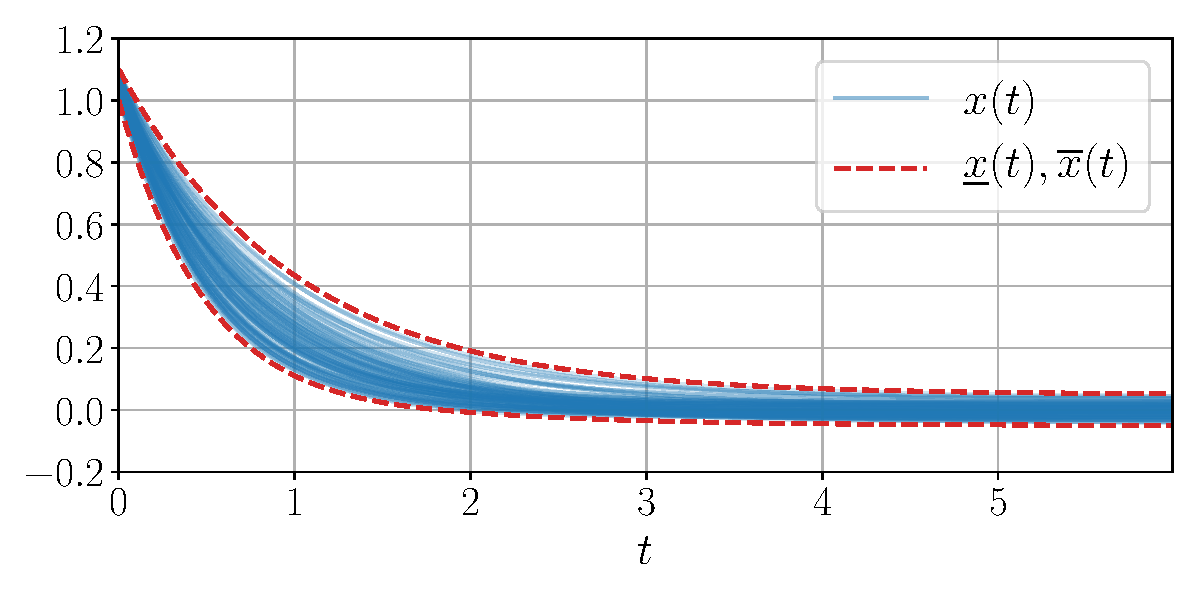
\includegraphics[width=\linewidth]{img/interval-predictor}
% \par\end{centering}
% \caption{Several trajectories for different values of $\theta\in\Theta$ are shown in blue. The result of prediction by \eqref{eq:interval-predictor} is in red: the predictor is stable and produces tight bounds.}
% \label{fig:predictor_example}
% \end{figure}
% \end{example*}

Limitations: set-based method assumes time-varying uncertainty where we have time-invariant uncertainty: $A(\theta)$ is fixed vs $A(\theta)$ can vary in $\cC_\delta$ at each step. Consequence: conservative overset.

\section{Control}

\label{sec:control}

\begin{definition}[Surrogate objective]
We approximate the robust objective $V^r$ in \eqref{eq:robust-control} by considering its interval prediction $[\underline{x}(t), \overline{x}(t)]$ based on the dynamics confidence region $\cC_\delta$:

\begin{align}
\underline{R}_n(\bu) \eqdef \min_{x\in[\underline{x}_n(\bu), \overline{x}_n(\bu)]}  R(x) \label{eq:pessimistic-rewards} \\
\hat{V}^r(\bu) \eqdef \sum_{n=N+1}^\infty \gamma^n \underline{R}_n(\bu) \label{eq:surrogate_objective}
\end{align}
where $\underline{x}_n(\bu), \overline{x}_n(\bu)$ follow the dynamics defined in \eqref{eq:interval-predictor}.
\end{definition}

This does not simply amounts to a change of reward function, since the worst case is assessed over the whole past trajectory being optimized, which means that this pessimistic reward $\underline{R_n}$ is not \emph{markovian}.

\begin{proposition}[Lower bound]
\label{prop:lower-bound}
With high probability, the surrogate objective $\hat{V}^r$ is a lower bound of the true objective $V^r$:

\begin{equation}
\hat{V}^r(\bu) \leq V^r(\bu)
\end{equation}
\end{proposition}

The consequence of \autoref{prop:lower-bound} is that since all our approximations were conservative, if we manage to find a control sequence such that no \textit{``bad event''} (e.g. a collision) happens according to the surrogate objective $\hat{V}^r$, then we are guaranteed so they will not happen either when the controls are executed on the true system. 

\paragraph{Planning}
In order to optimise $\hat{V}^r$, we turn to sequential planning algorithms. We cannot use Dynamic Programming algorithms because the state space is continuous and the pessimistic rewards are non-markovian. Instead, we turn to tree-based planning algorithms which optimise a sequence of actions based on the corresponding sequence of rewards. These methods no dot require the enumeration of the states nor the markovity of the rewards. In particular, we consider the \emph{Optimistic Planning of Deterministic Systems} (\texttt{OPD}) algorithm \citep{Hren2008} tailored for the case where the sequence of rewards is a deterministic function of the sequence of actions. Indeed, the stochasticity of the perturbations and measurements is encased in $\hat{V}^r$: both the predictor dynamics \eqref{eq:interval-predictor} and the corresponding pessimistic rewards \eqref{eq:pessimistic-rewards} are deterministic.

At each planning iteration $k\in[K]$, \texttt{OPD} progressively builds a tree $\cT_{k+1}$ by expanding the leaf $a_k$ with highest B-value, where the expansion of a leaf $a$ refers to the simulation of its children transitions $aA = \{ab, b\in A\}$:
\begin{equation}
\label{eq:opd}
a_k = \argmax_{a\in\cL_k} B_a(k), \quad B_a(k) = \sum_{n=0}^{h(a)-1} \underline{R}_n(a) + \frac{\gamma^{h(a)}}{1-\gamma}
\end{equation}
where $\cL_k$ is the set of leaves of $\cT_k$, $h(a)$ is the length of the sequence $a$, and $\underline{R}_n(a)$ the pessimistic reward \eqref{eq:pessimistic-rewards} obtained at time $n$ by following the sequence $a$.
\begin{theorem}[Planning performance, \citep{Hren2008}]
\label{theorem:opd-regret}
The simple regret of the \texttt{OPD} algorithm \eqref{eq:opd} after $K$ iterations is:
\begin{align*}
\text{if } \kappa>1,\quad& 
\hat{V}^r(a^*) - \hat{V}^r({a_K}) = \cO\left(K^{-\frac{\log 1/\gamma}{\log \kappa}}\right);\\
\text{if }\kappa=1,\quad&
\hat{V}^r(a^*) - \hat{V}^r({a_K}) = \cO\left(\gamma^{\frac{(1-\gamma)^\beta}{c}K}\right)
\end{align*}
where $\kappa$ is a problem-dependent measure of the proportion of near-optimal paths:
\[
\kappa = \limsup_{h\rightarrow\infty} \left|\left\{a\in A^h: \hat{V}^r(a)\geq \hat{V}^r - \frac{\gamma^{h+1}}{1-\gamma}\right\}\right|^{1/h}.
\]
\end{theorem}

Hence, by using enough computational budget $K$ for planning we can get as close as we want to the optimal surrogate value $\hat{V}^r(\bu^*)$, at a polynomial rate. However, there exists a gap between $\hat{V}^r$ and the true robust objective $V^r$, which stems from three approximations: (i) the true reachable set was approximated by an enclosing interval in \eqref{eq:inclusion-property}; (ii) the time-invariance of the dynamics uncertainty $A(\theta)\in\cC_{[N],\delta}$ was handled by the interval predictor \eqref{eq:interval-predictor} as if it were a time-varying uncertainty $\forall t, A(\theta(t))\in\cC_{[N],\delta}$ ; and (iii) the lower-bound $\sum\min\leq \min\sum$ used to define the surrogate objective \eqref{eq:surrogate_objective} is not tight.

However, under an additional smoothness assumption on $R$, we can bound this gap:
\begin{proposition}
\label{prop:control-error}
If the reward function $R$ is lipschitz, then the approximation error is upper-bounded by:
\begin{equation*}
     V^r(\bu) - \hat{V}^r(\bu) = \cO\left(\frac{1}{\sqrt{N}}\right)
\end{equation*}
\end{proposition}

% \begin{algorithm}[tb]
%   \caption{Robust Estimation, Prediction and Control (v1)}
%   \label{alg:full}
% \begin{algorithmic}
%   \STATE {\bfseries Input:} confidence level $\delta$
%   \FOR{$N = 1,2,3,\dots$} 
%   \STATE Compute the dynamics confidence region $\cC_{[N],\delta}$ with \textsc{Model Estimation} \eqref{eq:generic-polytope} on $\cD_{[N]}$.
%   \FOR{planning steps $k\in[K]$}
%   \STATE Get the tree node $\bu_k$ to expand with \textsc{Pessimistic Planning}  \eqref{eq:opd} using $\underline{R_n}$ over $[\underline{x}_{n}, \overline{x}_{n}]$. \COMMENT{Selection}
%   \STATE For each action, simulate the child transition $[\underline{x}_{n+1}, \overline{x}_{n+1}]$ with \textsc{Interval Prediction} \eqref{eq:interval-predictor} using $\cC_{[N],\delta}$. \COMMENT{Expansion}
%   \ENDFOR
%   \STATE Execute the first recommended control $u_N$, and add the observed transition $(x_N, u_N, \dot{x}_N)$ to $\cD_{[N+1]}$.
%   \ENDFOR
% \end{algorithmic}
% \end{algorithm}

\begin{algorithm}[tb]
	\caption{Robust Estimation, Prediction and Control}
	\label{alg:full}
	\begin{algorithmic}
		\STATE {\bfseries Input:} confidence level $\delta$
		\FOR{$N = 1,2,3,\dots$} 
		\STATE $\cC_{[N],\delta} \gets$\textsc{Model Estimation}$(\cD_{[N]})$. \eqref{eq:generic-polytope}
		\FOR{planning steps $k\in[K]$}
		\STATE $a_k\gets$\textsc{Pessimistic Planning}$(\underline{R_n}([\underline{x}_{n}, \overline{x}_{n}]))$.  \eqref{eq:opd}
		\FOR{$b\in A$}
		\STATE $[\underline{x}_{n+1}(a_k b), \overline{x}_{n+1}(a_k b)]\gets$ \textsc{Interval Prediction}($\cC_{[N],\delta}$). \eqref{eq:interval-predictor}
		\ENDFOR
		\ENDFOR
		\STATE Execute the first recommended control $u_N$, and add the observed transition $(x_N, u_N, \dot{x}_N)$ to $\cD_{[N+1]}$.
		\ENDFOR
	\end{algorithmic}
\end{algorithm}

\section{Multi-model Aggregation}

The procedure we developed in sections \ref{sec:estimation}, \ref{sec:prediction} and \ref{sec:control} relies on restrictive modelling assumptions, such as the linear dynamics \eqref{eq:dynamics} or \autoref{assumpt:structure}. But what if they are wrong?

\paragraph{Model adequacy}

One of the major benefits of using the family of linear models, compared to richer model classes, is that they provide strict conditions allowing to quantify the adequacy of the modelling assumptions to the observations.

TODO: from $\cC$ to confidence regions for $y_{n+1}$.

% Following \citep{maillard:hal-01349727}, we define the model adequacy for an observation $x(t), u(t), \dot{x}(t)$ of the modelling assumptions $(A, \phi)$ trained on history $\cD_{[N]}$ by:
% \begin{equation*}
%     \alpha(x(t), u(t), \dot{x}(t)) = \sup_\delta \argmin_{\delta\in(0,1)} d\left(\dot{x}(t), \cC_{[N],\delta}(x(t), u(t))\right)
% \end{equation*}
% where $d(\dot x,\cC(x,u)) = \inf_{\hat{A}\in\cC} \left\|\hat{A}x + Bu - \dot{x}\right\|^2 + \|\eta\|_\infty^2$.
% An adequacy of $0$ indicates a strong match of the assumptions, while an adequacy of $1$ indicates a strong mismatch. The 

This metric gets useful in the context of model selection and aggregation: 
This suggest using multiple models with different sets of features.

\subsection{Robust aggregation}

We temporarily ignore the parametric uncertainty over $\theta$ to simply consider several known candidate dynamics models, which all correspond to different modelling assumptions.

\begin{assumption}[Multi-model ambiguity]
\label{assumpt:multi-model-ambiguity}
Assume that the true dynamics $f$ lies within a finite set of candidate models $f^1, \cdots, f^M$.
\begin{equation}
\exists m\in[M]: \dot{x}(t) = f^M(x(t), u(t)), \forall t\geq 0
\end{equation}
\end{assumption}
We want to adapt our planning algorithm in order to aggregate these concurrent hypotheses in a robust fashion, i.e. maximise a robust objective with discrete ambiguity:
\[
V^r = \max_{\bu}\min_{m\in[M]} \sum_{t=1}^\infty \gamma^t R_t^m
\]
where $R_t^m$ is the reward obtain by following the sequence $\bu$ up to step $t$ under the dynamics $f^m$.

The traditional robust optimization procedures do not apply: Robust MDP: only with finite states (here continuous), and based on rectangular ambiguity. $\cH_\infty$ control also concern linear dynamics (which is not required under \autoref{assumpt:multi-model-ambiguity}) and .


\begin{definition}[Robust sequence upper bounds] We define an upper-bound for the value of a sequences of action $a$:
\begin{equation}
\label{eq:robust-b-values}
B_a^r(k)  \eqdef
\begin{cases}
\min_{m\in[M]} \sum_{n=0}^{h-1} \gamma^n R_n^m  + \frac{\gamma^h}{1-\gamma} &\text{if } a \text{ is a leaf;}\\
\max_{b\in\mathcal{A}} B_{ab}^r(k) & \text{else.}
\end{cases}
\end{equation}
where $R_t^m$ is the reward obtained at step $t$ by following $a$ with dynamics $f^m$.
\end{definition}
An illustration of the computation of the robust b-values is presented in Figure \ref{fig:drop}. From this definition we introduce Algorithm \ref{algo:drop}, and analyse its sample-efficiency in Theorem \ref{theorem:drop-regret}.

\begin{figure}
\centering
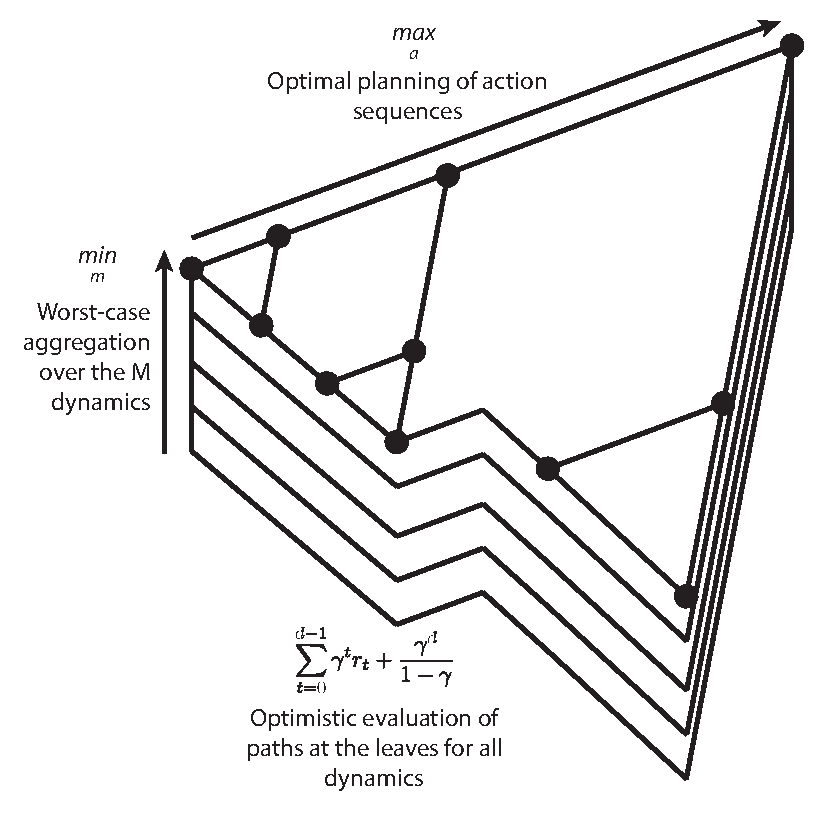
\includegraphics[width=0.4\linewidth]{img/robust-control-tree}
\caption{The computation of robust B-values in Algorithm \ref{algo:drop}. The simulation of trajectories for every dynamics model $f^m$ is represented as stacked versions of the expanded tree $\mathcal{T}_n$.}
\label{fig:drop}
\end{figure}

\begin{theorem}[Regret bound]
\label{theorem:drop-regret}
\texttt{ROPD} enjoys the same regret bound as provided for \texttt{OPD} in \autoref{theorem:opd-regret}.
\end{theorem}

The caveat is that $K$ measures the number of planning iterations, but actually expanding a node requires the simulation of $M$ time more transitions for each action than in the non-robust single-model setting.

\section{Experiments}


\paragraph{Obstacle avoidance with unknown friction}
We first consider a simple illustrative example: the control of a $2D$-
\paragraph{Behavioural planning for an autonomous vehicle}
We consider the problem of safe decision-making for an autonomous vehicle. An autonomous vehicle with state $\chi_0\in\Real^4$ is driving on a highway populated with $V$ other vehicles with states $\chi_i\in\Real^4$, resulting in a joint traffic state $x = [\chi_0, \chi_1,\dots,\chi_V]^\top\in\Real^{4V+4}$. In order to plan a sequence of high-level decisions, the autonomous agent relies on both a model of its own dynamics $\chi_0 = f_0(\chi_0,u)$, but also a parametrized dynamical model for each observed agent to predict their future trajectory: \[\dot{\chi}_i=f_i(x,\theta_i),\;i\in[V],\] where $f_i$ are described below, $\chi_i\in\Real^4$ is the state of an agent, $\theta_i\in\Real^5$ is the corresponding vector of unknown parameters. Crucially, this system $f$ describes the couplings and interactions between vehicles, so that the autonomous agent can properly anticipate their reactions. 
Already, we can appreciate a first advantage of the imposed structure \autoref{assumpt:structure}: the uncertainty space of $\theta$ is $\Real^{5V}$. In comparison, the traditional adaptive LQ setting where the whole state matrix $A$ is estimated would have resulted in a much larger parameter space $\theta\in\Real^{16V^2}$.
% In order to act safely in the face of uncertainty, we follow the framework of robust decision-making: the agent must consider all the possible trajectories in the space of $Z$ that each vehicle can follow in order to take its decisions.

The system 


\bibliography{references}
\bibliographystyle{icml2020}

\clearpage
\appendix

\section{Proofs}

\subsection{Proof of \autoref{prop:regularized_solution}}

\begin{proof}
We differentiate $J(\theta) = \sum_{n=1}^N \|y_n -\Phi_n\theta\|_{\Sigma_p^{-1}}^2 + \lambda\|\theta\|_{}^2$ as in  \eqref{eq:regression_min} with respect to $\theta$:

\begin{align*}
    \nabla_{\theta} J(\theta) &= \sum_{n=1}^N\nabla_{\theta} (y_n - \Phi_n\theta)^\transp\Sigma_p^{-1}(y_n - \Phi_n\theta) + \nabla_{\theta} \lambda\|\theta\|_{}^2\\
    &= -2\sum_{n=1}^N y_n^\transp\Sigma_p^{-1}\Phi_n + 2\sum_{n=1}^N\theta^\transp(\Phi_n^\transp\Sigma^{-1}\Phi_n) +  2 \lambda \theta^\transp
\end{align*}

Hence,
\begin{align*}
    \nabla_{\theta} J(\theta) = 0 \iff \left(\sum_{n=1}^N\Phi_n^\transp\Sigma_p^{-1}\Phi_n + I_d\right)\theta = \sum_{n=1}^N y_n^\transp\Sigma_p^{-1}\Phi_n
\end{align*}
\end{proof}

\subsection{Proof of \autoref{thm:confidence_ellipsoid}}

We start by showing a preliminary proposition:

\begin{proposition}[Theorem 1 of \citep{Abbasi2011}, Matrix version]
\label{prop:concentration}
Let $\{F_n\}_{n=0}$ be a filtration.
Let $\{\eta_n\}_{n=1}^\infty$ be a $\Real^p$-valued stochastic process such that $\eta_n$ is $F_n$-measurable and $\expectedvalue\left[\eta_n\condbar F_{n-1}\right]$ is $\Sigma_p$-sub-Gaussian.

Let $\{\Phi_n\}_{n=1}^\infty$ be an $\Real^{p\times d}$-valued stochastic process such that $\Phi_n$ is $F_n$-measurable. Assume that $G$ is a $d\times d$ positive definite matrix. For any $n\geq 0$, define:
\begin{equation*}
    \overline{G}_n = G + \sum_{s=1}^n \Phi_s^\transp \Sigma_p^{-1} \Phi_s \in \Real^{d\times d} \quad S_n = \sum_{s=1}^n \Phi_s^\transp\Sigma_p^{-1}\eta_s \in \Real^{d}.
\end{equation*}
Then, for any $\delta>0$, with probability at least $1-\delta$, for all $n\geq0$,
\begin{align*}
\| S_n \|_{\overline{G}_n^{-1}} \geq \sqrt{2\ln \left(\frac{\det\left(\overline{G}_n\right)^{1/2}}{\delta\det(G)^{1/2}}\right)}.
\end{align*}
\end{proposition}
\begin{proof}
Let 
\begin{equation*}
    G_t = \sum_{s=1}^t \Phi_s^\transp \Sigma_p^{-1} \Phi_s \in \Real^{d\times d}
\end{equation*}
And for any $z\in\Real^d$,
\begin{equation*}
    M_t^z = \exp{\left(\inp{z}{S_t} - \frac{1}{2}\|z\|_{G_t}\right)}
\end{equation*}
\begin{equation*}
    D_t^z = \exp{\left(\inp{\Phi_t z}{\eta_t}_{\Sigma_p^{-1}} - \frac{1}{2}\|\Phi_t z\|_{\Sigma_p^{-1}}\right)}
\end{equation*}
Then,
\begin{align*}
    M_t^z &= \exp{\left(\sum_{s=1}^t z^\transp \Phi_s^\transp \Sigma_p^{-1} \eta_s - \frac{1}{2} (\Phi_s z)^\transp\Sigma_p^{-1}(\Phi_s z) \right)} \\
    &= \prod_{s=1}^{t} D_s^z
\end{align*}
and using the Sub-Gaussianity of $\eta_t$
\begin{align*}
    \expectedvalue\left[D_t^z \condbar F_{t-1}\right] = {}& \exp{\left(- \frac{1}{2}\|\Phi_t z\|_{\Sigma_p^{-1}}\right)}\\ &\expectedvalue\left[\exp{\left(\inp{\Phi_t z}{\eta_t}_{\Sigma_p^{-1}}\right)} \condbar F_{t-1}\right]  \\
    \leq {} & \exp{\left(- \frac{1}{2}\|\Phi_t z\|_{\Sigma_p^{-1}}\right)}\\
    &\exp{\left((z^\transp \Phi_t^\transp \Sigma_p^{-1})\Sigma_p(\Sigma_p^{-1} \Phi_t z)\right)}\\
    &= 1
\end{align*}
\begin{align*}
    \expectedvalue\left[M_t^z \condbar F_{t-1}\right] = \left(\prod_{s=1}^{t-1} D_s^z\right) \expectedvalue\left[D_t^z \condbar F_{t-1}\right] \leq M_{t-1}^z
\end{align*}
Showing that $(M_t^z)_{t=1}^\infty$ is indeed a supermartingale and in fact $\expectedvalue[M_t^z]\leq 1$.
It then follows by Doob's upcrossing lemma for supermartingale that $M_\infty^z = \lim_{t\to\infty} M_t^z$ is almost surely well-defined, and so is $M_\tau^z$ for any random stopping time $\tau$.

Next, we consider the stopped martingale $M_{\min(\tau,t)}^z$. Since 
$(M_t^z)_{t=1}^\infty$ is a non-negative supermartingale and $\tau$ is a random stopping time, we deduce by Doob's decomposition that
\begin{align*}
\expectedvalue[M_{\min(\tau,t)}^z] &= \expectedvalue[M_0^z] + \expectedvalue[\sum_{s=0}^{t-1} (M_{s+1}^z-M_s^z) \mathbb{I}\{\tau>s\}]\\
&\leq 1 + \expectedvalue[\sum_{s=0}^{t-1} \expectedvalue[M_{s+1}^z-M_s^z|F_{s}] \mathbb{I}\{\tau>s\}]\\
&\leq 1
\end{align*}
Finally, an application of Fatou's lemma show that 
$\expectedvalue[M_\tau^z] = \expectedvalue[\liminf_{t\to\infty} M_{\min(\tau,t)}^z] \leq \liminf_{t\to\infty} \expectedvalue[M_{\min(\tau,t)}^z] \leq 1.$

\begin{lemma}[Theorem 14.7 of \citep{pena2008self}]
If $Z$ is a random vector and $B$ is a symmetric positive definite matrix such that
\[\forall \gamma\in\Real^d, \ln \expectedvalue \exp \left(\gamma^\transp Z -\frac{1}{2} \gamma^\transp B \gamma \right)\leq 0,\]
then for any positive definite non-random matrix C, it holds
\[\expectedvalue\left[ \sqrt{\frac{\det(C)}{\det(B+C)} } \exp\left( \frac{1}{2}\|Z\|^2_{(B+C)^{-1}}\right)\right]\leq 1. \] 
In particular, by Markov inequality, for all $\delta\in(0,1)$, 
\[\probability{\|Z\|_{(B+C)^{-1}} \geq \sqrt{2\ln \left(\frac{\det \left((B+C)^{1/2}\right)}{\delta\det(C)^{1/2}}\right)}}\leq \delta.\]
\end{lemma}

Here, by using $Z = \sum_{s=1}^t\Phi_s\Sigma_p^{-1}\eta_s$, $B=G_t$, $C=G$,

\[
\probability{\| S_t \|_{(G_t+G)^{-1}} \geq \sqrt{2\ln \left(\frac{\det(G_t+G)^{1/2}}{\delta\det(G)^{1/2}}\right)}} \leq \delta
\]

\end{proof}

Having shown this preliminary result, we move on to the proof of \autoref{thm:confidence_ellipsoid}.

\begin{proof}
For all $x\in\Real^d$, \eqref{eq:vector_rls} gives:
\begin{align*}
    x^\transp\theta_{N,\lambda}  -x^\transp\theta &= x^\transp G_{N, \lambda}^{-1}\sum_{n=1}^N \Phi_n^\transp \Sigma_p^{-1}\eta_n
    - \lambda x^\transp G_{N, \lambda}^{-1}\theta\\
    &= \inp{x}{\sum_{n=1}^N \Phi_n^\transp \Sigma_p^{-1}\eta_n}_{G_{N, \lambda}^{-1}} - \lambda\inp{x}{\theta}_{G_{N, \lambda}^{-1}}
\end{align*}

Using the Cauchy-Schwartz inequality, we get:
\begin{align*}
    |x^\transp\theta_{N,\lambda}  -x^\transp\theta| \leq {} & \|x\|_{G_{N, \lambda}^{-1}}\left(\left\|\sum_{n=1}^N \Phi_n^\transp \Sigma_p^{-1}\eta_n\right\|_{G_{N, \lambda}^{-1}}\right.\\ 
    &+ \left.\lambda\|\theta\|_{G_{N, \lambda}^{-1}}\right)
\end{align*}

In particular, for $x = G_{N,\lambda}(\theta_{N,\lambda} - \theta)$, we get after simplifying with $\| \theta_{N,\lambda}  - \theta\|_{G_{N,\lambda}}$:
\begin{align*}
    \| \theta_{N,\lambda}  - \theta\|_{G_{N,\lambda}} &\leq \left\|\sum_{n=1}^N \Phi_n^\transp \Sigma_p^{-1}\eta_n\right\|_{G_{N, \lambda}^{-1}} + \lambda\|\theta\|_{G_{N, \lambda}^{-1}}
\end{align*}

By applying \autoref{prop:concentration} with $G=\lambda I_d$, we obtain that with probability at least $1-\delta$,
\begin{align*}
    \| \theta_{N,\lambda}  - \theta\|_{G_{N,\lambda}} &\leq \sqrt{2\ln \left(\frac{\det(G_{N,\lambda})^{1/2}}{\delta\det(\lambda I_d)^{1/2}}\right)}
     + \lambda\|\theta\|_{G_{N, \lambda}^{-1}}
\end{align*}
And since $\|\theta\|_{G_{N, \lambda}^{-1}}^2 \leq 1/\lambda_{\min}(G_{N,\lambda})\|\theta\|_2^2 \leq 1/\lambda \|\theta\|_2^2$ and $\|\theta\|_2^2 \leq d\|\theta\|_\infty^2\leq d S^2$,
\begin{align*}
    \| \theta_{N,\lambda}  - \theta\|_{G_{N,\lambda}} &\leq \sqrt{2\ln \left(\frac{\det(G_{N,\lambda})^{1/2}}{\delta\det(\lambda I_d)^{1/2}}\right)}
     + (\lambda d)^{1/2}S
\end{align*}
\end{proof}


\subsection{Proof of \autoref{prop:lower-bound}}

\begin{proof}
	The predictor designed in \autoref{sec:prediction} verifies the inclusion property \eqref{eq:inclusion-property}. Thus, for sequence of controls $\bu$, any dynamics $A(\theta)\in C_{[N],\delta}$, and perturbations $\underline{\bw} \leq \bw \leq \overline{\bw}$, the corresponding state at time $t_n$ is bounded by $\underline{x}_n \leq x_n \leq \overline{x}_n$, which implies that $R(x_n) \geq \min_{x\in[\underline{x}_n(\bu), \overline{x}_n(\bu)]}  R(x) = \underline{R}_n(\bu)$.
	
	Thus, by taking the min over $C_{[N],\delta}$ and $[\underline{\bw}, \overline{\bw}]$, we also have for any sequence of controls $\bu$:
	\begin{align*}
	    V^r(\bu) &= \min_{\substack{A(\theta)\in C_{[N],\delta}\\ \underline{\bw} \leq \bw \leq \overline{\bw}}} \sum_{n=N+1}^\infty \gamma^n R(x_n)\\
	    &\geq \sum_{n=N+1}^\infty \gamma^n \underline{R}_n(\bu)\\
	    &= \hat{V}^r(\bu)
	\end{align*}
\end{proof}

\subsection{Proof of \autoref{prop:control-error}}

\begin{proof}
 By the inclusion property \eqref{eq:inclusion-property}, for any sequence of controls $\bu$, dynamics $A(\theta)\in C_{[N],\delta}$ and perturbations $\underline{\bw} \leq \bw \leq \overline{\bw}$, we have that $\underline{x}_n \leq x_n \leq \overline{x}_n$, which implies that $R(x_n) \leq \max_{x\in[\underline{x}_n(\bu), \overline{x}_n(\bu)]}  R(x)$.
 
 Thus, since we assume that $R$ is $L$-lipschitz,
 \begin{align}
     V^r(\bu) - \hat{V}^r(\bu) &\leq \sum_{n=N+1}^\infty \gamma^n \underset{{x\in[\underline{x}_n(\bu), \overline{x}_n(\bu)]}}{(\max - \min)} R(x)\\
     &\leq \sum_{n=N+1}^\infty \gamma^n L \left\|\underline{x}_n(\bu) - \overline{x}_n(\bu)\right\|
 \end{align}

\end{proof}


\subsection{Proof of \autoref{theorem:drop-regret}}

We start by showing the following lemma:


\begin{lemma}[Robust values ordering]
	In addition to the robust B-value defined in \eqref{eq:robust-b-values}, we also define the robust value of a sequence of actions $a$
	\begin{equation}
	V_a^r \eqdef \max_{\bu \in a\mathcal{A^\infty}} \min_{m\in[1, M]} \sum_{n=h(a)+1}^\infty \gamma^n R^m_n
	\end{equation}
	and the robust U-values of a sequence of action $a$
	\begin{equation}
	U_a^r(T)  \eqdef
	\begin{cases}
	\min_{m\in[M]} \sum_{n=0}^{h-1} \gamma^n R_n^m &\text{if } a \text{ is a leaf;}\\
	\max_{b\in\mathcal{A}} U_{ab}^r(n) & \text{else.}
	\end{cases}
	\end{equation}.
	
	Then, the robust values, U-values and B-values exhibit similar properties as the optimal values, U-values and B-values, that is: for all $0 < t < T$ and $a\in\mathcal{T}_T$,
	\begin{equation}
	U^r_a(t) \leq U^r_a(T) \leq V^r_a \leq B^r_a(T) \leq B^r_a(t)
	\end{equation}
	\label{lemma:uvb}
\end{lemma}
\begin{proof}
	By definition, when starting with sequence $i$, the value $u_i^m(n)$ represents the minimum admissible reward, while $b_i^m(n)$ corresponds to the best admissible reward achievable with respect to the the possible continuations of $i$. Thus, for all $i\in\mathcal{A}^*$, $u_i^m(n)$ and $u_i^r(n)$ are non-decreasing functions of $n$ and $b_i^m(n)$ and $b_i^r(n)$ are a non-increasing functions of $n$, while $v_i^m$ and $v_i^r$ do not depend on $n$.
	
	Moreover, since the reward function $r$ is assumed to have values in $[0, 1]$, the sum of discounted rewards from a node of depth $d$ is at most $\gamma^d + \gamma^{d+1}+\cdots = \frac{\gamma^d}{1-\gamma}$. As a consequence, for all $n \geq 0$ , $i\in\mathcal{L}_n$ of depth $d$, and any sequence of rewards $(r_t)_{t\in\mathbb{N}}$ obtained from following a path in $i\mathcal{A}^\infty$ with any dynamics $m \in [1, M]$:
	
	\begin{equation*}
	\sum_{t=0}^{d-1} \gamma^t r_t \leq \sum_{t=0}^{d-1} \gamma^t r_t + \sum_{t=d}^\infty \gamma^t r_t \leq \sum_{t=0}^{d-1} \gamma^t r_t + \frac{\gamma^d}{1-\gamma}
	\end{equation*}
	That is equivalent to:
	\begin{equation*}
	u^m_i(n) \leq \sum_{t=0}^\infty \gamma^t r_t \leq b^m_i(n) 
	\end{equation*}
	Hence,
	\begin{equation}
	\label{eq:min_m_values}
	\min_{m \in [1, M]} u^m_i(n) \leq \min_{m \in [1, M]} \sum_{t=0}^\infty \gamma^t r_t \leq \min_{m \in [1, M]} b^m_i(n)
	\end{equation}
	And as the left-hand and right-hand sides of \eqref{eq:min_m_values} are independent of the particular path that was followed in $i\mathcal{A}^\infty$, it also holds for the robust path:
	
	\begin{equation*}
	\min_{m \in [1, M]} u^m_i(n) \leq \max_{\pi\in i\mathcal{A}^\infty} \min_{m \in [1, M]} \sum_{t=0}^\infty \gamma^t r_t \leq \min_{m \in [1, M]} b^m_i(n)
	\end{equation*}
	that is,
	\begin{equation}
	\label{eq:urvrbr}
	u^r_i(n) \leq v^r_i  \leq b^r_i(n)
	\end{equation}
	
	Finally, \eqref{eq:urvrbr} is extended to the rest of $\mathcal{T}_n$ by recursive application of \eqref{eq:max_vr}, \eqref{eq:ur} and \eqref{eq:br}.
\end{proof}

We now turn to the proof of the theorem.

\begin{proof}
	\citet{Hren2008} first show in Theorem 2 that the simple regret of their optimistic planner is bounded by $\frac{\gamma^{d_n}}{1 - \gamma}$ where $d_n$ is the depth of $\mathcal{T}_n$. This properties relies on the fact that the returned action belongs to the deepest explored branch, which we can show likewise by contradiction using Lemma \ref{lemma:uvb}. This yields directly that $a = i_0$ where $i$ is some node of maximal depth $d_n$ expanded at round $t\leq n$, which by Algorithm \ref{algo:drop} verifies $b_a^r(t) = b_i^r(t) = \max_{x\in\mathcal{A}} b_x^r(t)$ and:
	\begin{align}
	\label{eq:Rndn}
	v^r - v_a^r &= v_{a^*}^r - v_a^r \\
	&\leq b_{a^*}^r(t) - v_a^r \\
	&\leq b_{a}^r(t) - u_a^r(t) \\
	&= b_{i}^r(t) - u_i^r(t) \\
	&= \frac{\gamma^{d_n}}{1-\gamma}.
	\end{align}
	
	Secondly, they bound the depth $d_n$ of $\mathcal{T}_n$ with respect to $n$. To that end, they show that the expanded nodes always belong to the sub-tree $\mathcal{T}_\infty$ of all the nodes of depth $d$ that are $\frac{\gamma^d}{1-\gamma}$-optimal. Indeed, if a node $i$ of depth $d$ is expanded at round $n$, then $b_i^r(n) \geq b_j^r(n)$ for all $j\in \mathcal{L}_n$ by Algorithm \ref{algo:drop}, thus the max-backups of \eqref{eq:br} up to the root yield $b^r_i(n) = b_\emptyset^r(n)$. Moreover, by Lemma \ref{lemma:uvb} we have that $b_\emptyset^r(n) \geq v_\emptyset^r = v^r$ and so $v_i^r \geq u_i^r(n) = b_i^r(n) - \frac{\gamma^d}{1-\gamma} \geq v^r - \frac{\gamma^d}{1-\gamma}$, thus $i \in \mathcal{T}_\infty$.
	
	Then from Assumption \ref{assumpt:beta} and the definition of $\beta$ applied to nodes in $\mathcal{T}_\infty$, there exists $d_0$ and $c$ such that the number $n_d$ of nodes of depth $d \geq d_0$ in $\mathcal{T}_\infty$ is bounded by $c\left(\frac{\gamma^d}{1-\gamma}\right)^\beta K^d$. As a consequence, 
	\begin{eqnarray*}
		n &= \sum_{d=0}^{d_n} n_d = n_0 + \sum_{d=d_0+1}^{d_n} n_d \\
		&\leq n_0 + \sum_{d=d_0+1}^{d_n} c\left(\frac{\gamma^d}{1-\gamma}\right)^\beta K^d \\
		&= n_0 + c'\sum_{d={d_0+1}}^{d_n} \kappa^d
	\end{eqnarray*}
	where $c'=\frac{c}{(1-\gamma)^\beta}$.
	
	\begin{itemize}
		\item If $\kappa > 1$, then $n \leq n_0 + c'\kappa^{d_0+1}\frac{\kappa^{d_n-d_0}-1}{\kappa-1}$ and thus $d_n \geq d_0 + \log_\kappa \frac{(n-n_0)(\kappa - 1)}{c'\kappa^{d_0+1}}$.
		We conclude from \eqref{eq:Rndn} that $\mathcal{R}_n \leq \frac{\gamma^{d_n}}{1-\gamma} = \frac{1}{1-\gamma} \left( \frac{(n-n_0)(\kappa - 1)}{c'\kappa^{d_0+1}} \right)^\frac{\log \gamma}{\log \kappa} = O\left(n^{-\frac{\log 1/\gamma}{\log \kappa}}\right)$.
		
		\item If $\kappa = 1$, then $n \leq n_0 + c'(d_n-d_0)$, hence from \eqref{eq:Rndn} we have $\mathcal{R}_n = O\left(\gamma^{nc'}\right)$.
	\end{itemize}
\end{proof}


\section{The use case of autonomous driving}

In the following, we describe the structure of the model representing the dynamics of of several vehicles driving and interacting with one another.

\subsection{Kinematics}

The kinematics of any vehicle $i\in\overline{1,V}$ are represented by the Kinematic Bicycle Model:
\begin{align}
	\dot{x}_i &= v_i\cos(\psi_i), \nonumber\\
	\dot{y}_i &= v_i\sin(\psi_i), \nonumber\\
	\dot{v}_i &= a_i, \nonumber\\
	\dot{\psi}_i &= \frac{v_i}{l}tan(\beta_i), \nonumber
\end{align}
where $(x_i, y_i)$ is the vehicle position, $v_i$ is its forward velocity and $\psi_i$ is its heading, $l$ is the vehicle half-length, $a_i$ is the acceleration command and $\beta_i$ is the slip angle at the centre of gravity, used as a steering command.

\subsection{Longitudinal control}
Longitudinal behaviour is modelled by a linear controller using three features inspired from the intelligent driver model (IDM) \cite{Treiber2000}: a desired velocity, a braking term to drive slower than the front vehicle, and a braking term to respect a safe distance to the front vehicle.

Denoting $f_i$ the index of the front vehicle preceding vehicle $i$, the acceleration command can be presented as follows:
\begin{equation*}
	a_i = \begin{bmatrix}
	\theta_{i,1} & \theta_{i,2} & \theta_{i,3}
	\end{bmatrix} \begin{bmatrix}
		v_0 - v_i \\
		-(v_{f_i}-v_i)^- \\
		-(x_{f_i} - x_i - (d_0 + v_iT))^- \\
	\end{bmatrix},
	\label{eq:theta_a}
\end{equation*}
where $v_0, d_0$ and $T$ respectively denote the speed limit, jam distance and time gap given by traffic rules.

\subsection{Lateral control}

The lane $L_i$ with the lateral position $y_{L_i}$ and heading $\psi_{L_i}$ is tracked by a cascade controller of lateral position and heading $\beta_i$, which is selected in a way the closed-loop dynamics take the form:

\begin{align}
	\label{eq:heading-command}
    \dot{\psi}_i &= \theta_{i,5}\left(\psi_{L_i}+\sin^{-1}\left(\frac{\tilde{v}_{i,y}}{v_i}\right)-\psi_i\right),\\
    \tilde{v}_{i,y} &= \theta_{i,4} (y_{L_i}-y_i). \nonumber
\end{align}
We assume that the drivers choose their steering command $\beta_i$ such that \eqref{eq:heading-command} is always achieved: $\beta_i = \tan^{-1}(\frac{l}{v_i}\dot{\psi}_i)$.

\subsection{LPV formulation}

The system presented so far is non-linear and must be cast into the LPV form. We approximate the non-linearities induced by the trigonometric operators through equilibrium linearisation around $y_i=y_{L_i}$ and $\psi_i=\psi_{L_i}$.

This yields the following longitudinal dynamics:
\begin{align*}
\dot{x}_i &= v_i,\\
\dot v_i &= \theta_{i,1} (v_0 - v_i) + \theta_{i,2} (v_{f_i} - v_i) + \theta_{i,3}(x_{f_i} - x_i - d_0 - v_i T),
\end{align*}
where $\theta_{i,2}$ and $\theta_{i,3}$ are set to $0$ whenever the corresponding features are not active.

It can be rewritten in the form $$\dot{Z} = A(\theta)(Z-Z_c) + d.$$ For example, in the case of two vehicles only:
\begin{equation*}
    Z = \begin{bmatrix}
x_i \\
x_{f_i} \\
v_i \\
v_{f_i} \\
\end{bmatrix}
,\quad
Z_c = \begin{bmatrix}
-d_0-v_0 T \\
0 \\
v_0\\
v_0 \\
\end{bmatrix}
,\quad
d = \begin{bmatrix}
v_0 \\
v_0 \\
0\\
0\\
\end{bmatrix}
\end{equation*}

\begin{equation*}
A(\theta)
=
\begin{blockarray}{ccccc}
 & i & f_i & i & f_i \\
\begin{block}{c[cccc]}
i & 0 & 0 & 1 & 0 \\
f_i & 0 & 0 & 0 & 1 \\
i & -\theta_{i,3} & \theta_{i,3} & -\theta_{i,1}-\theta_{i,2}-\theta_{i,3} & \theta_{i,2} \\
f_i & 0 & 0 & 0 & -\theta_{f_i,1} \\
\end{block}
\end{blockarray}
\end{equation*}

The lateral dynamics are in a similar form:
\begin{equation*}
\begin{bmatrix}
\dot{y}_i \\
\dot{\psi}_i \\
\end{bmatrix}
=
\begin{bmatrix}
0 & v_i \\
-\frac{\theta_{i,4} \theta_{i,5}}{v_i} & -\theta_{i,5}
\end{bmatrix}
\begin{bmatrix}
y_i - y_{L_i} \\
\psi_i - \psi_{L_i}
\end{bmatrix}
+
\begin{bmatrix}
v_i\psi_{L_i} \\
0
\end{bmatrix}
\end{equation*}
Here, the dependency in $v_i$ is seen as an uncertain parametric dependency, \emph{i.e.} $\theta_{i,6}=v_i$, with constant bounds assumed for $v_i$ using an overset of the longitudinal interval predictor.

\subsection{Tighter conversion form ellipsoid to polytope}
\label{sec:tight-polytope}
\begin{lemma}[Confidence polytope]
\label{lem:tight_polytope}
We can enclose the confidence ellipsoid obtained in $\eqref{eq:confidence-ellipsoid}$ within a polytope $C_\delta$:
\begin{equation}
     \cC_\delta = \left\{ A_{1}+\sum_{i=1}^{2^d}\lambda_{i}\Delta A_{i}: \lambda\in[0, 1]^{2^d},  \sum_{i=1}^{2^d}\lambda_{i}=1\right\}.
\end{equation}
with 
\begin{align*}
    &h_k \text{ is the }k^\text{th}\text{ element of }\{-1,1\}^d\text{ for } k\in[2^d],\\
    &G_{N,\lambda}^{-1} = PDP^{-1}, \quad \Delta\theta_k = C_{N,\lambda,\delta}^{1/2} P^{-1}D^{-1/2} h_k, \\
    &A_0 = A + \theta_{N,\lambda}^\transp\Phi, \quad \Delta A_k = \Delta\theta_k^\transp\Phi.
\end{align*}
This conversion is illustrated in \autoref{fig:ellipsoid_to_polytope}.
\end{lemma}

\begin{proof}
The ellipsoid in \eqref{eq:confidence-ellipsoid} is described by:
\begin{align*}
    \theta\in\cC_\delta &\implies
    (\theta-\theta_{N,\lambda})^\transp G_{N,\lambda}^{-1}(\theta-\theta_{N,\lambda}) \leq C_{N,\lambda,\delta}\\
    &\implies (\theta'-\theta'_{N,\lambda})^\transp D (\theta'-\theta'_{N,\lambda}) \leq C_{N,\lambda,\delta}\\
    &\implies \sum_{i=1}^d D_{i,i}(\theta'_i-\theta'_{N,\lambda,i})^2\leq C_{N,\lambda,\delta}\\
    &\implies\forall i, |\theta'_i-\theta'_{N,\lambda,i}|\leq C_{N,\lambda,\delta}^{1/2}D_{i,i}^{-1/2}
\end{align*}
This describes a $\Real^d$ box containing $\theta' = P\theta$, whose $k^\text{th}$ vertex is represented by $\theta_{N,\lambda}' + C_{N,\lambda,\delta}^{1/2}D^{-1/2} h_k$. We obtain the corresponding box on $\theta$ by transforming each vertex of the box with $P^{-1}$.
\end{proof}

\begin{figure}
    \centering
    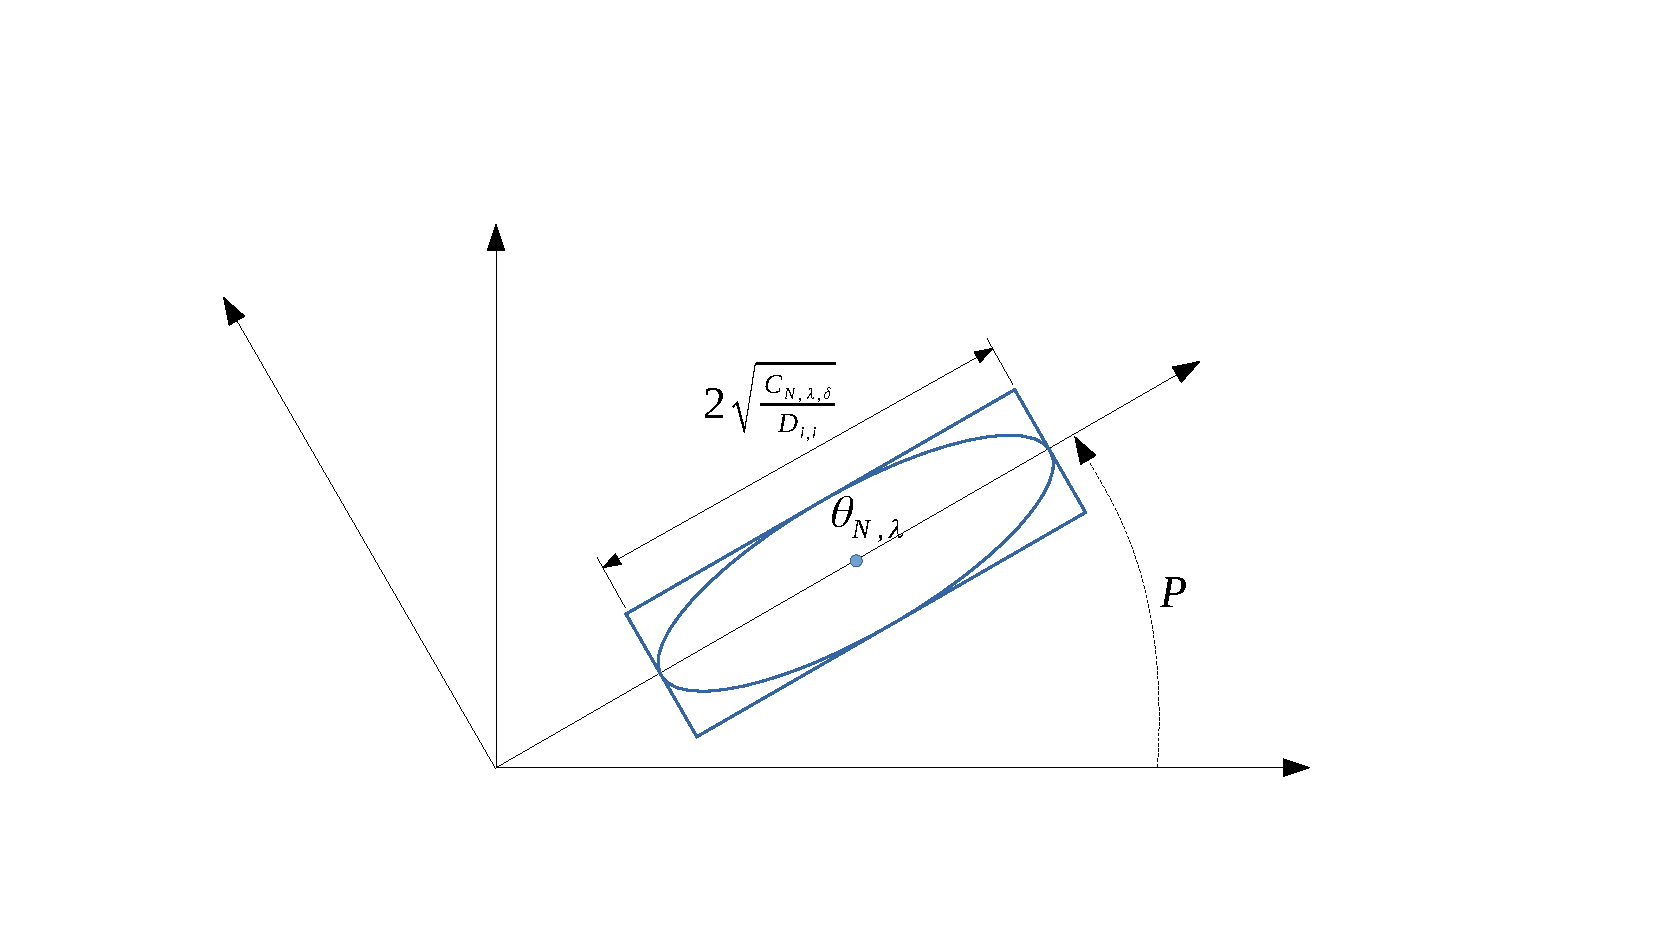
\includegraphics[trim={3.8cm, 2cm, 5cm, 3.8cm}, clip, width=0.4\textwidth]{img/ellipsoid_to_polytope}
    \caption{From the confidence ellipsoid $\cC_\delta$ to its enclosing polytope $\cP_\delta$}
    \label{fig:ellipsoid_to_polytope}
\end{figure}

\subsection{Change of coordinates}
In both cases, the obtained polytope centre $A_0$ is non-Metzler.
We use lemma \ref{lem:metzler} to compute a similarity transformation of coordinates. Precisely, we ensure that the polytope is chosen so that its centre $A_0$ is diagonalisable having real eigenvalues, and perform an eigendecomposition to compute its change of basis matrix $S$. The transformed system $Z'=S^{-1}(Z-Z_c)$ verifies \eqref{eq:polytope} with $A_0$ Metlzer as required to apply the interval predictor of Theorem~\ref{thm:predictor}. Finally, the obtained predictor is transformed back to the original coordinates $Z$ by using the interval arithmetic of Lemma~\ref{lem:interval}.


\end{document}
